\documentclass{SelimArticle}
\definecolor{RosyBrown}{rgb}{0.737255,0.560784,0.560784}
\definecolor{light goldenrod}{rgb}{0.933333,0.866667,0.509804}
\definecolor{LightGoldenrod}{rgb}{0.933333,0.866667,0.509804}
\definecolor{Sienna}{rgb}{0.627451,0.321569,0.176471}
\definecolor{Red}{rgb}{0.803922,0.000000,0.000000} %Actually red3

\sectionfont{ \sectionrule{0pt}{0pt}{-5pt}{0.8pt} }  %Horizontal line below section.
\setcounter{secnumdepth}{2}  % Numbering of sections and subsections
\usepackage{amsmath}
\usepackage{pdfpages}
\usepackage[refpage]{nomencl}
\usepackage{multirow}
\usepackage{bigstrut}
\usepackage{pdfpages}
\usepackage{setspace} %allows double spacing with \doublespacing command
\usepackage{pdflscape}
\usepackage[graphicx]{realboxes}
\setlength{\nomitemsep}{-\parsep}
\usepackage[linktoc=all]{hyperref} %allows me to make a hyperref table of contents
\hypersetup{
    colorlinks,
    citecolor=black,
    filecolor=black,
    linkcolor=black,
    urlcolor=black
}

%Used for nomenclature making
\renewcommand*{\pagedeclaration}[1]{\unskip\dotfill\hyperpage{#1}}
\makenomenclature
%In CMD, makeindex <filename>.nlo -s nomencl.ist -o <filename>.nls

%----------------------------------------------------------------------------------------
%	PACKAGES AND OTHER DOCUMENT CONFIGURATIONS
%----------------------------------------------------------------------------------------

\newcommand*{\plogo}{\fbox{$\mathcal{PL}$}} % Generic publisher logo

%----------------------------------------------------------------------------------------
%	TITLE PAGE
%----------------------------------------------------------------------------------------

\newcommand*{\titleAT}{\begingroup % Create the command for including the title page in the document
\newlength{\drop} % Command for generating a specific amount of whitespace
\drop=0.1\textheight % Define the command as 10% of the total text height

\rule{\textwidth}{1pt}\par % Thick horizontal line
\vspace{2pt}\vspace{-\baselineskip} % Whitespace between lines
\rule{\textwidth}{0.4pt}\par % Thin horizontal line

\vspace{\drop} % Whitespace between the top lines and title
\centering % Center all text
\textcolor{Red}{ % Red font color
{\Huge TERM PROJECT}\\[0.5\baselineskip] % Title line 1
{\Large MECH-530}\\[0.75\baselineskip] % Title line 2
{\Huge Progress Report 6}} % Title line 3

\vspace{0.25\drop} % Whitespace between the title and short horizontal line
\rule{0.3\textwidth}{0.4pt}\par % Short horizontal line under the title
\vspace{\drop} % Whitespace between the thin horizontal line and the author name

{\Large \textsc{Elaine Craigie} \\ \vspace{0.5cm} (260476434)}\par % Author name

\vfill % Whitespace between the author name and publisher text
%{\large \textcolor{Red}{\plogo}}\\[0.5\baselineskip] % Publisher logo

\includegraphics[scale = 0.45]{pic_mcgill}
\vspace{2.0cm}
{\Large \\ \today}\par % Publisher
\vspace{1.0cm}
{\raggedleft{}
\textcolor{Red}{
{\large \\ \textsc{Overview:} This progress report features the optimization of three design problems using the code that has been developed.}}}
\centering
\rule{\textwidth}{0.4pt}\par % Thin horizontal line
\vspace{2pt}\vspace{-\baselineskip} % Whitespace between lines
\rule{\textwidth}{1pt}\par % Thick horizontal line

\endgroup}

%----------------------------------------------------------------------------------------
%	BLANK DOCUMENT
%----------------------------------------------------------------------------------------
\begin{document}
\numberwithin{figure}{section}
\numberwithin{table}{section}
\pagestyle{empty} % Removes page numbers

\titleAT % This command includes the title page
%%%%%%%%%%%%%%%%%%%%

\printnomenclature[0.5in]
\newpage
\pagenumbering{arabic}
\setcounter{page}{1}
\section{Design 1: Design of a Filament Wound Pressure Vessel}
Based on the following given parameters, the applied load vectors were obtained. Thus, $N_{1} = 0.025~\text{MN/m}$ and $N_{2} = 0.05~\text{MN/m}$ (tensile loads) while $N_{6} = 0$~N/m, and $M_{1} = M_{2} = M_{6} = 0$~N.
\begin{itemize}
\item p = 1.25 MPa (pressure inside the cylinder)
\item D = 8.0 cm (width/diameter of the cylinder)
\end{itemize}
\begin{align*}
N_{1} &= \bar{\sigma_{1}} \cdot h \\
&= \frac{p \cdot D}{4} \\
&= \frac{1.25 \cdot 10^{6} \cdot 0.08}{4} \\
&= 0.025 \cdot 10^{6}~\text{N/m}
\end{align*}
\begin{align*} 
N_{2} &= \bar{\sigma_{2}} \cdot h \\
&= \frac{p \cdot D}{2} \\
&= \frac{1.25 \cdot 10^{6} \cdot 0.08}{2} \\
&= 0.050 \cdot 10^{6}~\text{N/m}
\end{align*}
Thus the optimal ply angle for the layup $[\pm\theta]_{s}$ is for $\theta = 52^{o}$. This was determined from Figure~\ref{fig:q1graph}~since this value maximizes the Hashin R.
\begin{figure}[H]
        \centering
        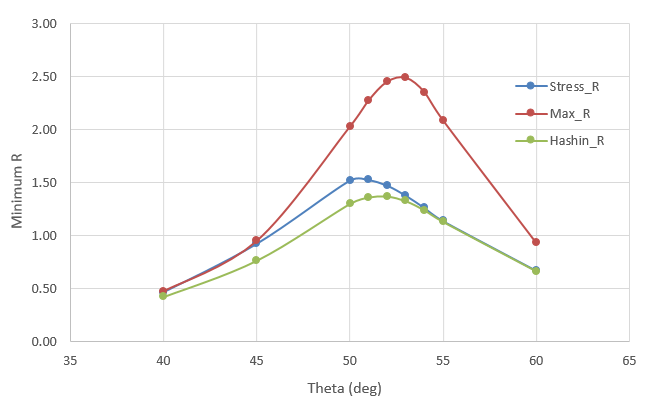
\includegraphics[width=0.7\textwidth]{q1_graph}
        \caption{Optimization of R Values for Various $\theta$}
        \label{fig:q1graph}
\end{figure}
Refer to Tables~\ref{tab:q1stress}~and~\ref{tab:q1r}~in Appendix~\ref{sec:q1} for the program output as well as the stresses, strains and safety factor $R$ values per top and bottom of each ply.

\section{Design 2: Design of a Laminate}
Generally $D_{11} = D_{22}$ for a balanced angle ply with $\theta = 45^{o}$.

In this case, no load is applied and the layup given in Table~\ref{tab:q2},~(also written [55/-25/-55/25]$_{s}$), produces a constant of proportionality $D_{11}/D_{22} = K = 0.9375$ which satisfies the given design requirements. Thus a total of 8 layers are used and the laminate is symmetric. Please refer to the output in Appendix~\ref{sec:q2} for further details.
\begin{table}[H]
\centering
\caption{Layup for Design 2}
\label{tab:q2}
\begin{tabular}{|c|c|c|c|c|}
\hline
Ply & Qty             & Material           & Angle & Thickness \\
& & & ($^{o}$) & (mm) \\
\hline
        8 &          1 & E-glass/Epoxy &         55 &      0.125 \\

        7 &          1 & E-glass/Epoxy &        -25 &      0.125 \\

        6 &          1 & E-glass/Epoxy &        -55 &      0.125 \\

        4-5 &          2 & E-glass/Epoxy &         25 &      0.250 \\

        3 &          1 & E-glass/Epoxy &        -55 &      0.125 \\

        2 &          1 & E-glass/Epoxy &        -25 &      0.125 \\

        1 &          1 & E-glass/Epoxy &         55 &      0.125 \\
\hline
\end{tabular}  
\end{table}  

\section{Design 3: Design of a Hockey Stick Blade}
\begin{table}[H]
\centering
\caption{Layup for Design 3}
\label{tab:q3finallayup}
\begin{tabular}{|c|c|c|c|c|}
\hline
Ply & Qty             & Material           & Angle & Thickness \\
& & & ($^{o}$) & (mm) \\
\hline
        17 &          1 & T300/N5208 &          0 &      0.125 \\

        16 &          1 & T300/N5208 &         10 &      0.125 \\

        15 &          1 & T300/N5208 &         17 &      0.125 \\

        14 &          1 & T300/N5208 &        -17 &      0.125 \\

        13 &          1 & T300/N5208 &         37 &      0.125 \\

        12 &          1 & T300/N5208 &        -37 &      0.125 \\

        11 &          1 & T300/N5208 &         35 &      0.125 \\

        10 &          1 & T300/N5208 &         13 &      0.125 \\

         9 &          1 &       CORE &        N/A &        1.5 \\

         8 &          1 & T300/N5208 &         13 &      0.125 \\

         7 &          1 & T300/N5208 &         35 &      0.125 \\

         6 &          1 & T300/N5208 &        -37 &      0.125 \\

         5 &          1 & T300/N5208 &         37 &      0.125 \\

         4 &          1 & T300/N5208 &        -17 &      0.125 \\

         3 &          1 & T300/N5208 &         17 &      0.125 \\

         2 &          1 & T300/N5208 &         10 &      0.125 \\

         1 &          1 & T300/N5208 &          0 &      0.125 \\
\hline
\end{tabular}  
\end{table}
The highest compressive loads (both moments and in-plane) are in the 1-axis. To optimize strength, the fiber directions should remain as close to $0^o$~as possible to combat this; however, there are also loads in the 2 and 3 axes, so a unidirectional laminate is not the solution.

After trial and error, the symmetric layup that meets the requirements is given by Table~\ref{tab:q3finallayup}, also written [0/10/$\pm$17/$\pm$37/35/13/C$_{1/2}$]$_{s}$~, where the corresponding minimum safety factors for each of the failure criterion are listed in Table~\ref{tab:q3finalR}.

From Engineering Toolbox, the approximate density of Balsa Wood is $\rho = 160~\text{kg/m}^{3}$. Thus, the core represents an added weight of 0.72~g to the laminate, as shown below. 
\begin{align*}
m_{core} &= \rho \cdot W \cdot B \cdot h_{o} \\
&= 160 \cdot 0.03 \cdot 0.1 \cdot 0.0015 \\
&= 7.2 \cdot 10^{-4}~\text{kg} \\
&= 0.72~\text{g}
\end{align*} 
This layup thus has a total of 17 plies with a mass of 10.32~g, (both of which include the core). The mass without the core is 9.60~g.

Refer to Tables~\ref{tab:q3stress1},~\ref{tab:q3r1},~\ref{tab:q3stress2}~and~\ref{tab:q3r2}~in Appendix~\ref{sec:q3} for the program output as well as the stresses, strains and safety factor $R$ values per top and bottom of each ply.
\begin{table}[H]
\centering
\caption{Minimum Safety Factors for Load Cases 1 and 2} \label{tab:q3finalR}
\begin{tabular}{|c|ccc|}
\hline
           & \multicolumn{ 3}{|c|}{Failure Criterion} \\
\hline
 Load Case & Maximum Stress &  Quadratic &     Hashin \\
\hline
         1 &      2.204 &      2.162 &      2.204 \\

         2 &      2.260 &      2.188 &      2.260 \\
\hline
\end{tabular} 
\end{table} 
 	
\newpage
\appendix
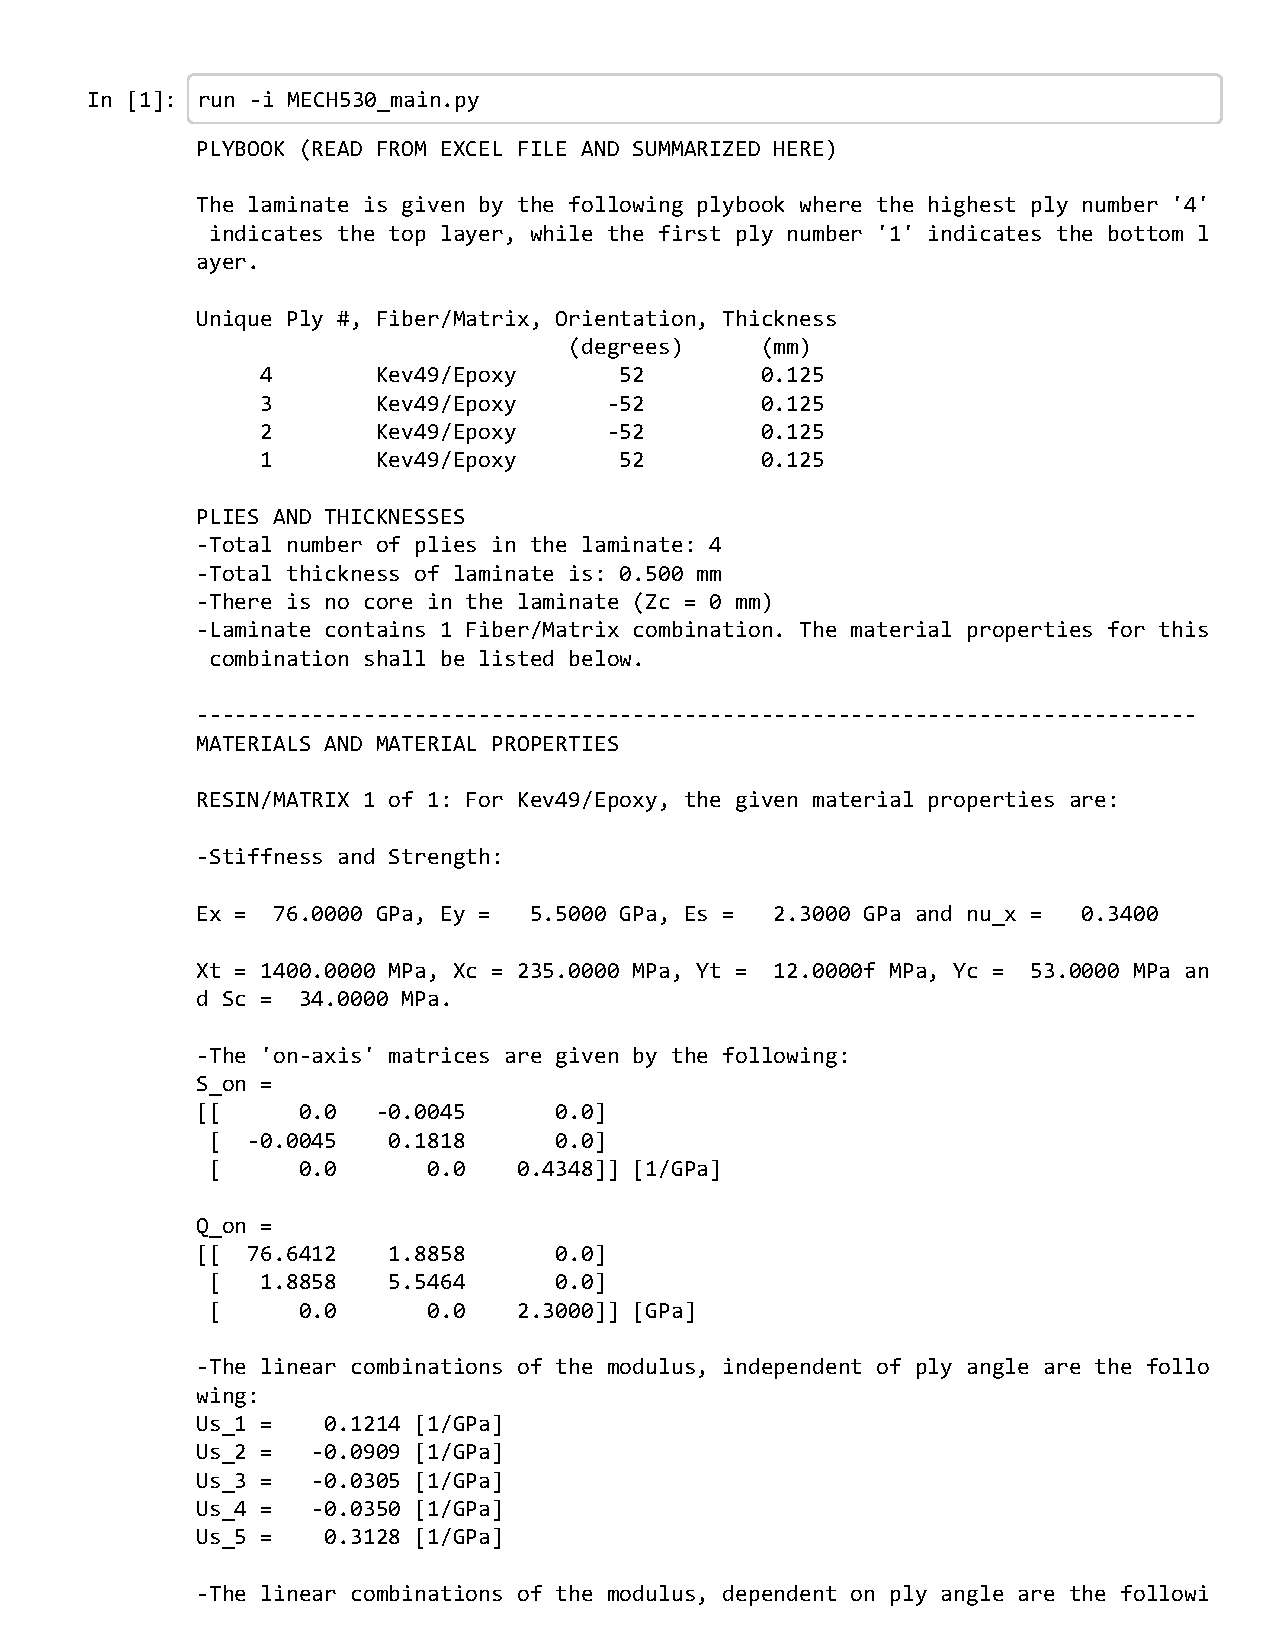
\includepdf[pages={1},scale=0.9,pagecommand={\section{Design 1 Output}\label{sec:q1}\thispagestyle{empty}}]{q1_notebook.pdf}
\includepdf[pages={2-}]{q1_notebook.pdf}

\begin{landscape}
\begin{table}
\centering
\caption{Design 1 Stress and Strain Values}
\label{tab:q1stress}
\begin{tabular}{|ccc|ccc|ccc|ccc|}
\toprule
Position &  Ply &  Angle & $\epsilon_{1}$ & $\epsilon_{2}$ & $\epsilon_{6}$ & $\epsilon_{x}$ & $\epsilon_{y}$ & $\epsilon_{s}$ & $\sigma_{x}$ & $\sigma_{y}$ & $\sigma_{s}$ \\
\midrule
 & & ($^{o}$) & & & & & & & (GPa) & (GPa) & (GPa) \\
\midrule
TOP &    4 &     52 & -0.0007 &  0.003375 &    0 &  0.00183 &  0.000844 &  0.003954 &       0.141865 &       0.008135 &       0.009094 \\
BOT &    4 &     52 & -0.0007 &  0.003375 &    0 &  0.00183 &  0.000844 &  0.003954 &       0.141865 &       0.008135 &       0.009094 \\
TOP &    3 &    -52 & -0.0007 &  0.003375 &    0 &  0.00183 &  0.000844 & -0.003954 &       0.141865 &       0.008135 &      -0.009094 \\
BOT &    3 &    -52 & -0.0007 &  0.003375 &    0 &  0.00183 &  0.000844 & -0.003954 &       0.141865 &       0.008135 &      -0.009094 \\
TOP &    2 &    -52 & -0.0007 &  0.003375 &    0 &  0.00183 &  0.000844 & -0.003954 &       0.141865 &       0.008135 &      -0.009094 \\
BOT &    2 &    -52 & -0.0007 &  0.003375 &    0 &  0.00183 &  0.000844 & -0.003954 &       0.141865 &       0.008135 &      -0.009094 \\
TOP &    1 &     52 & -0.0007 &  0.003375 &    0 &  0.00183 &  0.000844 &  0.003954 &       0.141865 &       0.008135 &       0.009094 \\
BOT &    1 &     52 & -0.0007 &  0.003375 &    0 &  0.00183 &  0.000844 &  0.003954 &       0.141865 &       0.008135 &       0.009094 \\
\bottomrule
\end{tabular}
\end{table}

\begin{table}
\centering
\caption{Design 1 Failure Criterion R Values}
\label{tab:q1r}
\begin{tabular}{|ccc|ccccc|cc|cccc|}
\toprule
 & & & \multicolumn{5}{|c|}{Maximum Stress} & \multicolumn{2}{|c|}{Quad Poly} & \multicolumn{4}{|c|}{Hashin Criterion} \\
\midrule
Position & Ply & Angle & FT & FC & MT & MC & S & (+) & (-) & FT & FC & MT & MC \\
\midrule
TOP & 4 &  52 &   9.869 &   0.000 &   1.475 &   0.000 &  3.739 & 2.455 & -2.595 &    3.496 &    0.000 &    1.372 &    0.000 \\
BOT & 4 &  52 &   9.869 &   0.000 &   1.475 &   0.000 &  3.739 & 2.455 & -2.595 &    3.496 &    0.000 &    1.372 &    0.000 \\
TOP & 3 & -52 &   9.869 &   0.000 &   1.475 &   0.000 &  3.739 & 2.455 & -2.595 &    3.496 &    0.000 &    1.372 &    0.000 \\
BOT & 3 & -52 &   9.869 &   0.000 &   1.475 &   0.000 &  3.739 & 2.455 & -2.595 &    3.496 &    0.000 &    1.372 &    0.000 \\
TOP & 2 & -52 &   9.869 &   0.000 &   1.475 &   0.000 &  3.739 & 2.455 & -2.595 &    3.496 &    0.000 &    1.372 &    0.000 \\
BOT & 2 & -52 &   9.869 &   0.000 &   1.475 &   0.000 &  3.739 & 2.455 & -2.595 &    3.496 &    0.000 &    1.372 &    0.000 \\
TOP & 1 &  52 &   9.869 &   0.000 &   1.475 &   0.000 &  3.739 & 2.455 & -2.595 &    3.496 &    0.000 &    1.372 &    0.000 \\
BOT & 1 &  52 &   9.869 &   0.000 &   1.475 &   0.000 &  3.739 & 2.455 & -2.595 &    3.496 &    0.000 &    1.372 &    0.000 \\
\bottomrule
\end{tabular}
\end{table}
\end{landscape}
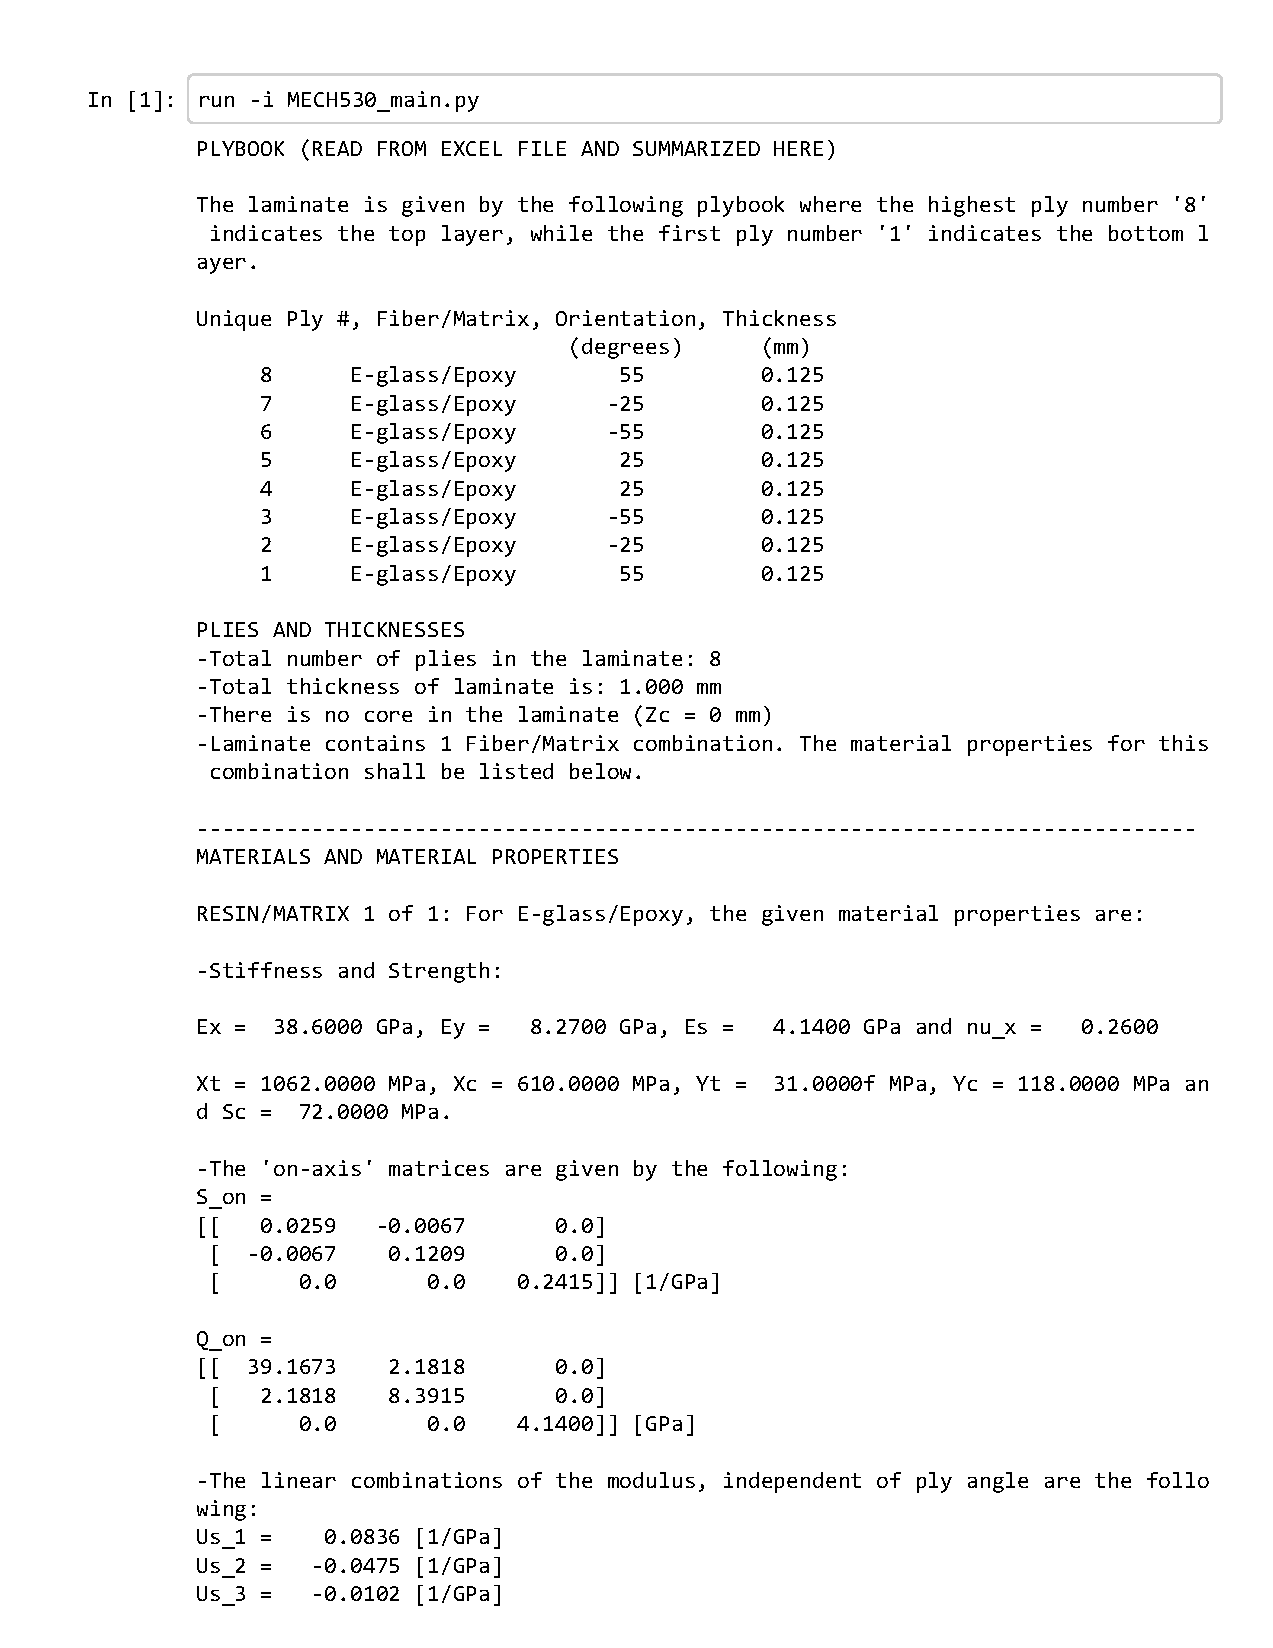
\includepdf[pages={1},scale=0.9,pagecommand={\section{Design 2 Output}\label{sec:q2}\thispagestyle{empty}}]{q2_notebook.pdf}
\includepdf[pages={2-}]{q2_notebook.pdf}

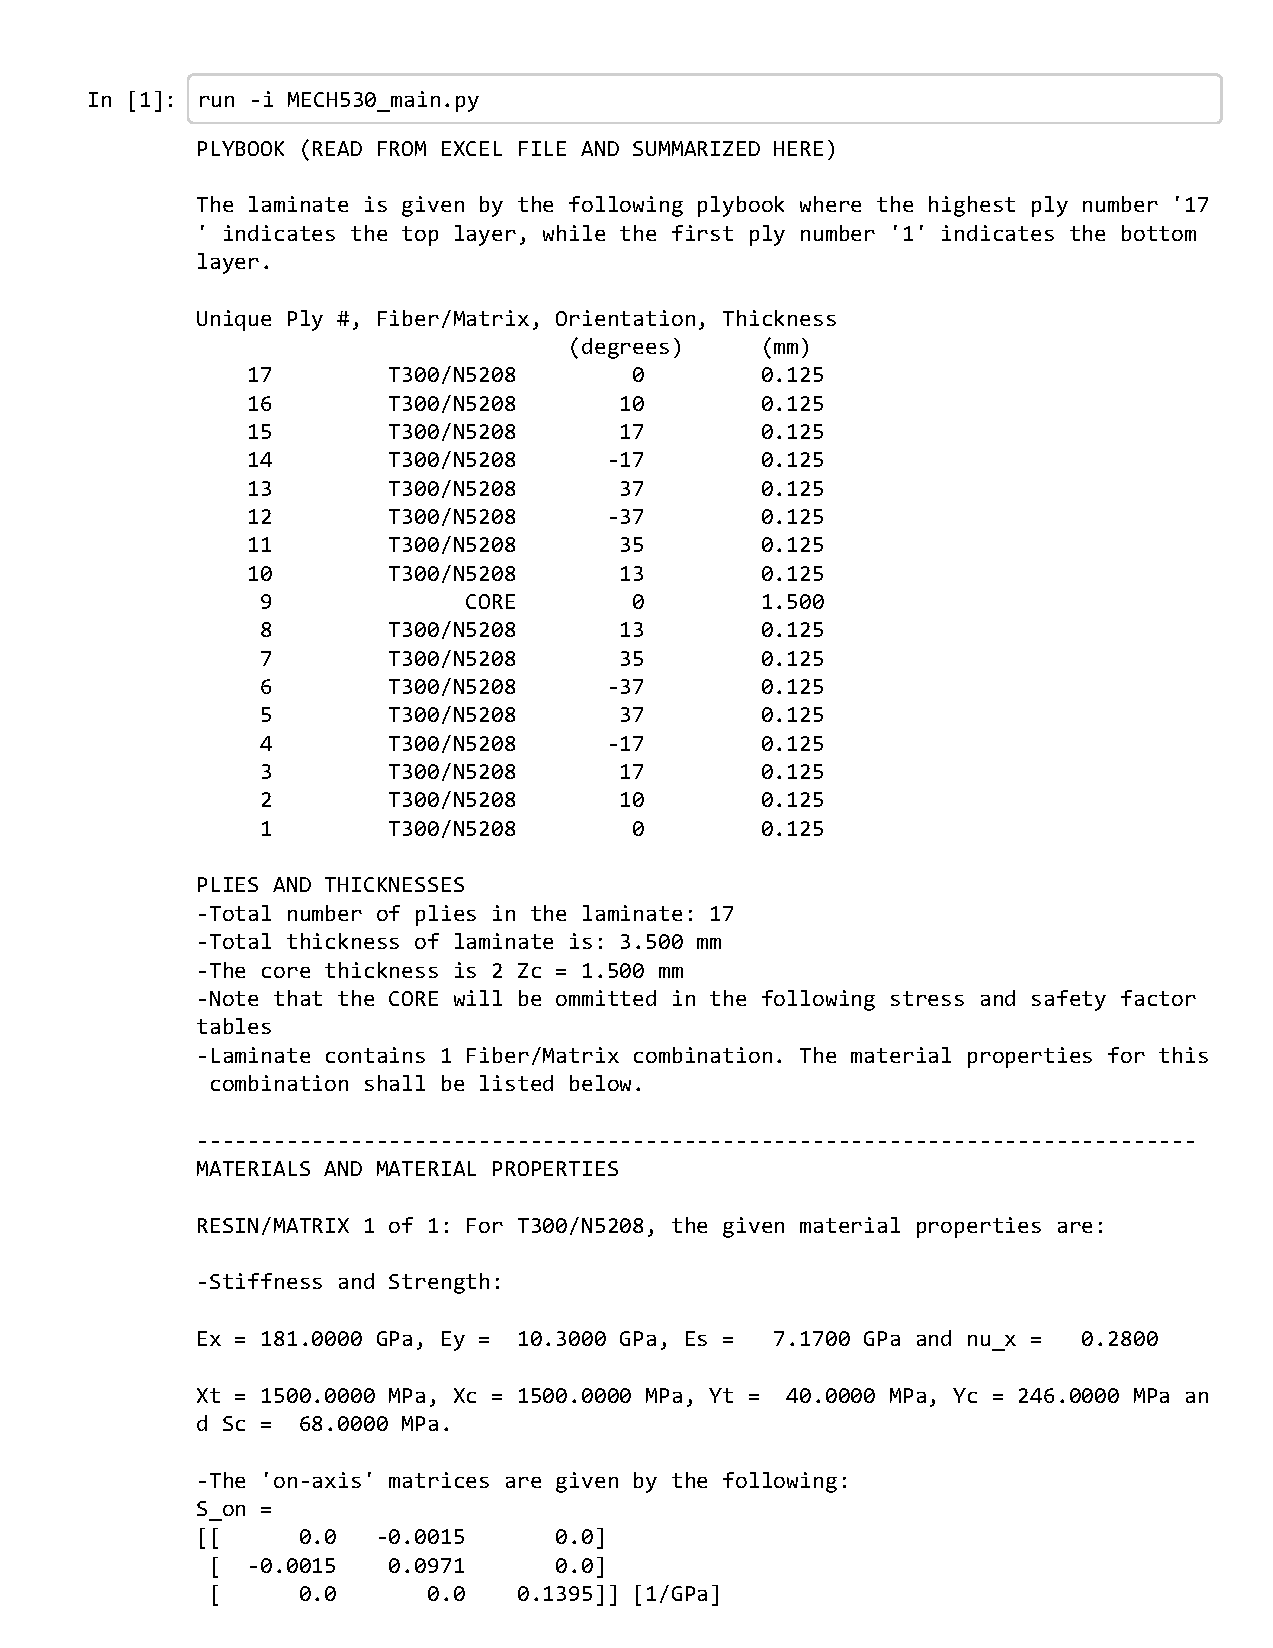
\includepdf[pages={1},scale=0.9,pagecommand={\section{Design 3 Output}\label{sec:q3}\thispagestyle{empty}}]{q3_notebook.pdf}
\includepdf[pages={2-}]{q3_notebook.pdf}

\begin{landscape}
\begin{table}
\centering
\caption{Design 3 Stress and Strain Values: Load Case 1}
\label{tab:q3stress1}
\begin{tabular}{|ccc|ccc|ccc|ccc|}
\toprule
Position &  Ply &  Angle & $\epsilon_{1}$ & $\epsilon_{2}$ & $\epsilon_{6}$ & $\epsilon_{x}$ & $\epsilon_{y}$ & $\epsilon_{s}$ & $\sigma_{x}$ & $\sigma_{y}$ & $\sigma_{s}$ \\
\midrule
 & & ($^{o}$) & & & & & & & (GPa) & (GPa) & (GPa) \\
\midrule
TOP &   17 &      0 & -0.003754 &  0.000622 & -0.000420 & -0.003754 &  0.000622 & -0.000420 &      -0.680662 &      -0.004437 &      -0.003013 \\
BOT &   17 &      0 & -0.003492 &  0.000579 & -0.000390 & -0.003492 &  0.000579 & -0.000390 &      -0.633147 &      -0.004128 &      -0.002795 \\
TOP &   16 &     10 & -0.003492 &  0.000579 & -0.000390 & -0.003436 &  0.000523 &  0.001026 &      -0.623113 &      -0.004546 &       0.007356 \\
BOT &   16 &     10 & -0.003230 &  0.000535 & -0.000359 & -0.003178 &  0.000483 &  0.000950 &      -0.576313 &      -0.004208 &       0.006812 \\
TOP &   15 &     17 & -0.003230 &  0.000535 & -0.000359 & -0.003008 &  0.000314 &  0.001807 &      -0.546026 &      -0.005469 &       0.012959 \\
BOT &   15 &     17 & -0.002968 &  0.000492 & -0.000329 & -0.002764 &  0.000288 &  0.001662 &      -0.501658 &      -0.005029 &       0.011915 \\
TOP &   14 &    -17 & -0.002968 &  0.000492 & -0.000329 & -0.002580 &  0.000104 & -0.002207 &      -0.468766 &      -0.006398 &      -0.015823 \\
BOT &   14 &    -17 & -0.002706 &  0.000448 & -0.000298 & -0.002353 &  0.000095 & -0.002011 &      -0.427449 &      -0.005832 &      -0.014417 \\
TOP &   13 &     37 & -0.002706 &  0.000448 & -0.000298 & -0.001707 & -0.000551 &  0.002949 &      -0.311899 &      -0.010643 &       0.021146 \\
BOT &   13 &     37 & -0.002444 &  0.000405 & -0.000268 & -0.001541 & -0.000498 &  0.002664 &      -0.281562 &      -0.009619 &       0.019100 \\
TOP &   12 &    -37 & -0.002444 &  0.000405 & -0.000268 & -0.001283 & -0.000756 & -0.002811 &      -0.235508 &      -0.011536 &      -0.020158 \\
BOT &   12 &    -37 & -0.002181 &  0.000361 & -0.000237 & -0.001147 & -0.000674 & -0.002509 &      -0.210415 &      -0.010294 &      -0.017992 \\
TOP &   11 &     35 & -0.002181 &  0.000361 & -0.000237 & -0.001457 & -0.000364 &  0.002308 &      -0.265866 &      -0.007985 &       0.016548 \\
BOT &   11 &     35 & -0.001919 &  0.000317 & -0.000207 & -0.001281 & -0.000321 &  0.002031 &      -0.233773 &      -0.007034 &       0.014564 \\
TOP &   10 &     13 & -0.001919 &  0.000317 & -0.000207 & -0.001852 &  0.000250 &  0.000795 &      -0.335912 &      -0.002782 &       0.005698 \\
BOT &   10 &     13 & -0.001657 &  0.000274 & -0.000176 & -0.001598 &  0.000215 &  0.000688 &      -0.289967 &      -0.002408 &       0.004934 \\
TOP &    8 &     13 &  0.001487 & -0.000248 &  0.000190 &  0.001441 & -0.000202 & -0.000590 &       0.261371 &       0.002082 &      -0.004233 \\
BOT &    8 &     13 &  0.001749 & -0.000292 &  0.000220 &  0.001694 & -0.000237 & -0.000697 &       0.307315 &       0.002456 &      -0.004997 \\
TOP &    7 &     35 &  0.001749 & -0.000292 &  0.000220 &  0.001181 &  0.000276 & -0.001843 &       0.215521 &       0.006278 &      -0.013213 \\
BOT &    7 &     35 &  0.002011 & -0.000336 &  0.000251 &  0.001357 &  0.000319 & -0.002119 &       0.247614 &       0.007229 &      -0.015197 \\
TOP &    6 &    -37 &  0.002011 & -0.000336 &  0.000251 &  0.001041 &  0.000635 &  0.002325 &       0.191066 &       0.009583 &       0.016669 \\
BOT &    6 &    -37 &  0.002273 & -0.000379 &  0.000281 &  0.001177 &  0.000717 &  0.002627 &       0.216158 &       0.010825 &       0.018836 \\
TOP &    5 &     37 &  0.002273 & -0.000379 &  0.000281 &  0.001448 &  0.000446 & -0.002472 &       0.264498 &       0.008813 &      -0.017725 \\
BOT &    5 &     37 &  0.002535 & -0.000423 &  0.000312 &  0.001614 &  0.000499 & -0.002757 &       0.294835 &       0.009837 &      -0.019771 \\
TOP &    4 &    -17 &  0.002535 & -0.000423 &  0.000312 &  0.002195 & -0.000083 &  0.001912 &       0.398888 &       0.005504 &       0.013711 \\
BOT &    4 &    -17 &  0.002797 & -0.000466 &  0.000342 &  0.002423 & -0.000092 &  0.002108 &       0.440205 &       0.006071 &       0.015118 \\
TOP &    3 &     17 &  0.002797 & -0.000466 &  0.000342 &  0.002614 & -0.000283 & -0.001541 &       0.474427 &       0.004646 &      -0.011051 \\
BOT &    3 &     17 &  0.003059 & -0.000510 &  0.000373 &  0.002858 & -0.000309 & -0.001687 &       0.518794 &       0.005086 &      -0.012095 \\
TOP &    2 &     10 &  0.003059 & -0.000510 &  0.000373 &  0.003015 & -0.000466 & -0.000871 &       0.546886 &       0.003916 &      -0.006242 \\
BOT &    2 &     10 &  0.003321 & -0.000553 &  0.000403 &  0.003273 & -0.000505 & -0.000946 &       0.593686 &       0.004255 &      -0.006786 \\
TOP &    1 &      0 &  0.003321 & -0.000553 &  0.000403 &  0.003321 & -0.000553 &  0.000403 &       0.602257 &       0.003898 &       0.002890 \\
BOT &    1 &      0 &  0.003583 & -0.000597 &  0.000434 &  0.003583 & -0.000597 &  0.000434 &       0.649773 &       0.004207 &       0.003108 \\
\bottomrule
\end{tabular}
\end{table}

\begin{table}
\centering
\caption{Design 3 Failure Criterion Safety Factor $R$ Values: Load Case 1}
\label{tab:q3r1}
\begin{tabular}{|ccc|ccccc|cc|cccc|}
\toprule
 & & & \multicolumn{5}{|c|}{Maximum Stress} & \multicolumn{2}{|c|}{Quad Poly} & \multicolumn{4}{|c|}{Hashin Criterion} \\
\midrule
Position & Ply & Angle & FT & FC & MT & MC & S & (+) & (-) & FT & FC & MT & MC \\
\midrule
TOP  & 17 &   0 &   0.000 &   2.204 &   0.000 &  55.442 & 22.568 & 2.555 & -2.065 &    0.000 &    2.204 &    0.000 &   26.158 \\
BOT  & 17 &   0 &   0.000 &   2.369 &   0.000 &  59.588 & 24.333 & 2.747 & -2.220 &    0.000 &    2.369 &    0.000 &   28.193 
\\
TOP  & 16 &  10 &   0.000 &   2.407 &   0.000 &  54.112 &  9.245 & 2.746 & -2.177 &    0.000 &    2.407 &    0.000 &   10.621 \\
BOT & 16 &  10 &   0.000 &   2.603 &   0.000 &  58.465 &  9.983 & 2.969 & -2.353 &    0.000 &    2.603 &    0.000 &   11.468 \\
TOP & 15 &  17 &   0.000 &   2.747 &   0.000 &  44.984 &  5.247 & 2.971 & -2.217 &    0.000 &    2.747 &    0.000 &    5.843 \\
BOT & 15 &  17 &   0.000 &   2.990 &   0.000 &  48.918 &  5.707 & 3.234 & -2.413 &    0.000 &    2.990 &    0.000 &    6.355 \\
TOP  & 14 & -17 &   0.000 &   3.200 &   0.000 &  38.447 &  4.297 & 3.251 & -2.265 &    0.000 &    3.200 &    0.000 &    4.769 \\
BOT  & 14 & -17 &   0.000 &   3.509 &   0.000 &  42.184 &  4.717 & 3.566 & -2.485 &    0.000 &    3.509 &    0.000 &    5.234 \\
TOP  & 13 &  37 &   0.000 &   4.809 &   0.000 &  23.115 &  3.216 & 3.776 & -2.051 &    0.000 &    4.809 &    0.000 &    3.633 \\
BOT & 13 &  37 &   0.000 &   5.327 &   0.000 &  25.575 &  3.560 & 4.182 & -2.270 &    0.000 &    5.327 &    0.000 &    4.022 \\
TOP & 12 & -37 &   0.000 &   6.369 &   0.000 &  21.324 &  3.373 & 4.365 & -2.125 &    0.000 &    6.369 &    0.000 &    3.851 \\
BOT & 12 & -37 &   0.000 &   7.129 &   0.000 &  23.898 &  3.779 & 4.890 & -2.381 &    0.000 &    7.129 &    0.000 &    4.315 \\
TOP & 11 &  35 &   0.000 &   5.642 &   0.000 &  30.807 &  4.109 & 4.627 & -2.609 &    0.000 &    5.642 &    0.000 &    4.626 \\
BOT & 11 &  35 &   0.000 &   6.416 &   0.000 &  34.972 &  4.669 & 5.260 & -2.964 &    0.000 &    6.416 &    0.000 &    5.257 \\
TOP & 10 &  13 &   0.000 &   4.465 &   0.000 &  88.437 & 11.934 & 4.998 & -3.871 &    0.000 &    4.465 &    0.000 &   13.448 \\
BOT & 10 &  13 &   0.000 &   5.173 &   0.000 & 102.179 & 13.782 & 5.790 & -4.482 &    0.000 &    5.173 &    0.000 &   15.529 \\
TOP &  8 &  13 &   5.739 &   0.000 &  19.215 &   0.000 & 16.063 & 5.019 & -6.423 &    5.404 &    0.000 &   12.324 &    0.000 \\
BOT &  8 &  13 &   4.881 &   0.000 &  16.288 &   0.000 & 13.608 & 4.265 & -5.463 &    4.594 &    0.000 &   10.443 &    0.000 \\
TOP &  7 &  35 &   6.960 &   0.000 &   6.372 &   0.000 &  5.147 & 3.270 & -5.736 &    4.138 &    0.000 &    4.004 &    0.000 \\
BOT &  7 &  35 &   6.058 &   0.000 &   5.534 &   0.000 &  4.475 & 2.843 & -4.991 &    3.599 &    0.000 &    3.479 &    0.000 \\
TOP &  6 & -37 &   7.851 &   0.000 &   4.174 &   0.000 &  4.079 & 2.570 & -5.305 &    3.620 &    0.000 &    2.917 &    0.000 \\
BOT &  6 & -37 &   6.939 &   0.000 &   3.695 &   0.000 &  3.610 & 2.274 & -4.694 &    3.203 &    0.000 &    2.582 &    0.000 \\
TOP &  5 &  37 &   5.671 &   0.000 &   4.539 &   0.000 &  3.836 & 2.450 & -4.472 &    3.178 &    0.000 &    2.930 &    0.000 \\
BOT &  5 &  37 &   5.088 &   0.000 &   4.066 &   0.000 &  3.439 & 2.197 & -4.011 &    2.849 &    0.000 &    2.626 &    0.000 \\
TOP &  4 & -17 &   3.760 &   0.000 &   7.267 &   0.000 &  4.959 & 2.641 & -3.797 &    2.996 &    0.000 &    4.096 &    0.000 \\
BOT &  4 & -17 &   3.408 &   0.000 &   6.589 &   0.000 &  4.498 & 2.394 & -3.442 &    2.716 &    0.000 &    3.715 &    0.000 \\
TOP &  3 &  17 &   3.162 &   0.000 &   8.609 &   0.000 &  6.153 & 2.567 & -3.422 &    2.812 &    0.000 &    5.006 &    0.000 \\
BOT &  3 &  17 &   2.891 &   0.000 &   7.865 &   0.000 &  5.622 & 2.347 & -3.129 &    2.571 &    0.000 &    4.574 &    0.000 \\
TOP &  2 &  10 &   2.743 &   0.000 &  10.214 &   0.000 & 10.894 & 2.489 & -3.127 &    2.660 &    0.000 &    7.451 &    0.000 \\
BOT &  2 &  10 &   2.527 &   0.000 &   9.401 &   0.000 & 10.021 & 2.292 & -2.880 &    2.450 &    0.000 &    6.856 &    0.000 \\
TOP &  1 &   0 &   2.491 &   0.000 &  10.262 &   0.000 & 23.531 & 2.333 & -2.881 &    2.477 &    0.000 &    9.406 &    0.000 \\
BOT &  1 &   0 &   2.308 &   0.000 &   9.509 &   0.000 & 21.876 & 2.162 & -2.671 &    2.296 &    0.000 &    8.720 &    0.000 \\
\bottomrule
\end{tabular}
\end{table}
\end{landscape}


\begin{landscape}
\begin{table}
\centering
\caption{Design 3 Stress and Strain Values: Load Case 2}
\label{tab:q3stress2}
\begin{tabular}{|ccc|ccc|ccc|ccc|}
\toprule
Position &  Ply &  Angle & $\epsilon_{1}$ & $\epsilon_{2}$ & $\epsilon_{6}$ & $\epsilon_{x}$ & $\epsilon_{y}$ & $\epsilon_{s}$ & $\sigma_{x}$ & $\sigma_{y}$ & $\sigma_{s}$ \\
\midrule
 & & ($^{o}$) & & & & & & & (GPa) & (GPa) & (GPa) \\
\midrule
TOP &   17 &      0 & -0.003661 &  0.000719 & -0.000744 & -0.003661 &  0.000719 & -0.000744 &      -0.663574 &      -0.003164 &      -0.005332 \\
BOT &   17 &      0 & -0.003406 &  0.000674 & -0.000691 & -0.003406 &  0.000674 & -0.000691 &      -0.617318 &      -0.002892 &      -0.004955 \\
TOP &   16 &     10 & -0.003406 &  0.000674 & -0.000691 & -0.003401 &  0.000669 &  0.000746 &      -0.616447 &      -0.002928 &       0.005350 \\
BOT &   16 &     10 & -0.003151 &  0.000629 & -0.000638 & -0.003146 &  0.000624 &  0.000693 &      -0.570201 &      -0.002656 &       0.004968 \\
TOP &   15 &     17 & -0.003151 &  0.000629 & -0.000638 & -0.003006 &  0.000484 &  0.001584 &      -0.545186 &      -0.003698 &       0.011361 \\
BOT &   15 &     17 & -0.002896 &  0.000584 & -0.000586 & -0.002762 &  0.000450 &  0.001460 &      -0.500890 &      -0.003344 &       0.010469 \\
TOP &   14 &    -17 & -0.002896 &  0.000584 & -0.000586 & -0.002435 &  0.000123 & -0.002431 &      -0.442283 &      -0.005785 &      -0.017433 \\
BOT &   14 &    -17 & -0.002641 &  0.000539 & -0.000533 & -0.002220 &  0.000118 & -0.002220 &      -0.403251 &      -0.005212 &      -0.015917 \\
TOP &   13 &     37 & -0.002641 &  0.000539 & -0.000533 & -0.001745 & -0.000357 &  0.002909 &      -0.318376 &      -0.008746 &       0.020859 \\
BOT &   13 &     37 & -0.002386 &  0.000493 & -0.000481 & -0.001574 & -0.000318 &  0.002635 &      -0.287056 &      -0.007852 &       0.018893 \\
TOP &   12 &    -37 & -0.002386 &  0.000493 & -0.000481 & -0.001112 & -0.000780 & -0.002900 &      -0.204406 &      -0.011293 &      -0.020793 \\
BOT &   12 &    -37 & -0.002130 &  0.000448 & -0.000428 & -0.000991 & -0.000691 & -0.002597 &      -0.182134 &      -0.010023 &      -0.018619 \\
TOP &   11 &     35 & -0.002130 &  0.000448 & -0.000428 & -0.001483 & -0.000199 &  0.002277 &      -0.270223 &      -0.006355 &       0.016325 \\
BOT &   11 &     35 & -0.001875 &  0.000403 & -0.000375 & -0.001302 & -0.000170 &  0.002013 &      -0.237220 &      -0.005532 &       0.014430 \\
TOP &   10 &     13 & -0.001875 &  0.000403 & -0.000375 & -0.001842 &  0.000370 &  0.000661 &      -0.333868 &      -0.001508 &       0.004742 \\
BOT &   10 &     13 & -0.001620 &  0.000358 & -0.000323 & -0.001591 &  0.000329 &  0.000577 &      -0.288267 &      -0.001209 &       0.004138 \\
TOP &    8 &     13 &  0.001442 & -0.000184 &  0.000309 &  0.001427 & -0.000170 & -0.000435 &       0.258947 &       0.002380 &      -0.003121 \\
BOT &    8 &     13 &  0.001697 & -0.000229 &  0.000361 &  0.001678 & -0.000211 & -0.000520 &       0.304548 &       0.002679 &      -0.003726 \\
TOP &    7 &     35 &  0.001697 & -0.000229 &  0.000361 &  0.001233 &  0.000235 & -0.001686 &       0.224815 &       0.005999 &      -0.012091 \\
BOT &    7 &     35 &  0.001952 & -0.000275 &  0.000414 &  0.001414 &  0.000264 & -0.001951 &       0.257818 &       0.006822 &      -0.013986 \\
TOP &    6 &    -37 &  0.001952 & -0.000275 &  0.000414 &  0.000947 &  0.000731 &  0.002254 &       0.174223 &       0.010303 &       0.016163 \\
BOT &    6 &    -37 &  0.002207 & -0.000320 &  0.000466 &  0.001068 &  0.000820 &  0.002557 &       0.196495 &       0.011573 &       0.018337 \\
TOP &    5 &     37 &  0.002207 & -0.000320 &  0.000466 &  0.001516 &  0.000371 & -0.002300 &       0.276716 &       0.008233 &      -0.016493 \\
BOT &    5 &     37 &  0.002462 & -0.000365 &  0.000519 &  0.001688 &  0.000410 & -0.002574 &       0.308036 &       0.009127 &      -0.018459 \\
TOP &    4 &    -17 &  0.002462 & -0.000365 &  0.000519 &  0.002075 &  0.000022 &  0.002011 &       0.377390 &       0.006239 &       0.014420 \\
BOT &    4 &    -17 &  0.002717 & -0.000410 &  0.000572 &  0.002290 &  0.000017 &  0.002223 &       0.416423 &       0.006811 &       0.015937 \\
TOP &    3 &     17 &  0.002717 & -0.000410 &  0.000572 &  0.002610 & -0.000303 & -0.001275 &       0.473617 &       0.004430 &      -0.009141 \\
BOT &    3 &     17 &  0.002972 & -0.000455 &  0.000624 &  0.002854 & -0.000337 & -0.001399 &       0.517912 &       0.004784 &      -0.010032 \\
TOP &    2 &     10 &  0.002972 & -0.000455 &  0.000624 &  0.002976 & -0.000459 & -0.000586 &       0.539714 &       0.003876 &      -0.004199 \\
BOT &    2 &     10 &  0.003228 & -0.000500 &  0.000677 &  0.003231 & -0.000504 & -0.000639 &       0.585961 &       0.004148 &      -0.004581 \\
TOP &    1 &      0 &  0.003228 & -0.000500 &  0.000677 &  0.003228 & -0.000500 &  0.000677 &       0.585363 &       0.004173 &       0.004853 \\
BOT &    1 &      0 &  0.003483 & -0.000546 &  0.000730 &  0.003483 & -0.000546 &  0.000730 &       0.631619 &       0.004445 &       0.005231 \\
\bottomrule
\end{tabular}
\end{table}

\begin{table}
\centering
\caption{Design 3 Failure Criterion Safety Factor $R$ Values: Load Case 2}
\label{tab:q3r2}
\begin{tabular}{|ccc|ccccc|cc|cccc|}
\toprule
 & & & \multicolumn{5}{|c|}{Maximum Stress} & \multicolumn{2}{|c|}{Quad Poly} & \multicolumn{4}{|c|}{Hashin Criterion} \\
\midrule
Position & Ply & Angle & FT & FC & MT & MC & S & (+) & (-) & FT & FC & MT & MC \\
\midrule
TOP  & 17 &   0 &   0.000 &   2.260 &   0.000 &  77.752 & 12.754 & 2.484 & -2.133 &    0.000 &    2.260 &    0.000 &   14.604 \\
BOT  & 17 &   0 &   0.000 &   2.430 &   0.000 &  85.057 & 13.725 & 2.665 & -2.295 &    0.000 &    2.430 &    0.000 &   15.696 \\
TOP & 16 &  10 &   0.000 &   2.433 &   0.000 &  84.005 & 12.710 & 2.665 & -2.291 &    0.000 &    2.433 &    0.000 &   14.458 \\
BOT  & 16 &  10 &   0.000 &   2.631 &   0.000 &  92.612 & 13.687 & 2.874 & -2.478 &    0.000 &    2.631 &    0.000 &   15.540 \\
TOP & 15 &  17 &   0.000 &   2.751 &   0.000 &  66.527 &  5.986 & 2.876 & -2.352 &    0.000 &    2.751 &    0.000 &    6.534 \\
BOT  & 15 &  17 &   0.000 &   2.995 &   0.000 &  73.557 &  6.495 & 3.121 & -2.561 &    0.000 &    2.995 &    0.000 &    7.081 \\
TOP  & 14 & -17 &   0.000 &   3.391 &   0.000 &  42.527 &  3.901 & 3.155 & -2.283 &    0.000 &    3.391 &    0.000 &    4.264 \\
BOT & 14 & -17 &   0.000 &   3.720 &   0.000 &  47.199 &  4.272 & 3.449 & -2.506 &    0.000 &    3.720 &    0.000 &    4.666 \\
TOP & 13 &  37 &   0.000 &   4.711 &   0.000 &  28.128 &  3.260 & 3.597 & -2.169 &    0.000 &    4.711 &    0.000 &    3.628 \\
BOT  & 13 &  37 &   0.000 &   5.225 &   0.000 &  31.329 &  3.599 & 3.968 & -2.402 &    0.000 &    5.225 &    0.000 &    4.003 \\
TOP & 12 & -37 &   0.000 &   7.338 &   0.000 &  21.783 &  3.270 & 4.288 & -2.129 &    0.000 &    7.338 &    0.000 &    3.718 \\
BOT & 12 & -37 &   0.000 &   8.236 &   0.000 &  24.544 &  3.652 & 4.780 & -2.387 &    0.000 &    8.236 &    0.000 &    4.149 \\
TOP & 11 &  35 &   0.000 &   5.551 &   0.000 &  38.708 &  4.165 & 4.375 & -2.765 &    0.000 &    5.551 &    0.000 &    4.609 \\
BOT & 11 &  35 &   0.000 &   6.323 &   0.000 &  44.471 &  4.712 & 4.944 & -3.144 &    0.000 &    6.323 &    0.000 &    5.207 \\
TOP & 10 &  13 &   0.000 &   4.493 &   0.000 & 163.156 & 14.339 & 4.736 & -4.120 &    0.000 &    4.493 &    0.000 &   15.626 \\
BOT & 10 &  13 &   0.000 &   5.204 &   0.000 & 203.520 & 16.435 & 5.440 & -4.782 &    0.000 &    5.204 &    0.000 &   17.805 \\
TOP &  8 &  13 &   5.793 &   0.000 &  16.809 &   0.000 & 21.787 & 5.126 & -6.883 &    5.598 &    0.000 &   13.308 &    0.000 \\
BOT &  8 &  13 &   4.925 &   0.000 &  14.932 &   0.000 & 18.250 & 4.373 & -5.794 &    4.755 &    0.000 &   11.557 &    0.000 \\
TOP &  7 &  35 &   6.672 &   0.000 &   6.668 &   0.000 &  5.624 & 3.423 & -6.003 &    4.300 &    0.000 &    4.299 &    0.000 \\
BOT &  7 &  35 &   5.818 &   0.000 &   5.863 &   0.000 &  4.862 & 2.979 & -5.184 &    3.731 &    0.000 &    3.743 &    0.000 \\
TOP &  6 & -37 &   8.610 &   0.000 &   3.882 &   0.000 &  4.207 & 2.556 & -5.695 &    3.780 &    0.000 &    2.853 &    0.000 \\
BOT &  6 & -37 &   7.634 &   0.000 &   3.456 &   0.000 &  3.708 & 2.263 & -5.010 &    3.336 &    0.000 &    2.528 &    0.000 \\
TOP &  5 &  37 &   5.421 &   0.000 &   4.859 &   0.000 &  4.123 & 2.569 & -4.610 &    3.282 &    0.000 &    3.144 &    0.000 \\
BOT &  5 &  37 &   4.870 &   0.000 &   4.383 &   0.000 &  3.684 & 2.304 & -4.116 &    2.938 &    0.000 &    2.820 &    0.000 \\
TOP &  4 & -17 &   3.975 &   0.000 &   6.411 &   0.000 &  4.716 & 2.614 & -3.969 &    3.039 &    0.000 &    3.799 &    0.000 \\
BOT &  4 & -17 &   3.602 &   0.000 &   5.872 &   0.000 &  4.267 & 2.372 & -3.584 &    2.752 &    0.000 &    3.452 &    0.000 \\
TOP &  3 &  17 &   3.167 &   0.000 &   9.029 &   0.000 &  7.439 & 2.669 & -3.547 &    2.914 &    0.000 &    5.741 &    0.000 \\
BOT &  3 &  17 &   2.896 &   0.000 &   8.362 &   0.000 &  6.778 & 2.442 & -3.233 &    2.663 &    0.000 &    5.266 &    0.000 \\
TOP &  2 &  10 &   2.779 &   0.000 &  10.320 &   0.000 & 16.192 & 2.561 & -3.233 &    2.739 &    0.000 &    8.703 &    0.000 \\
BOT &  2 &  10 &   2.560 &   0.000 &   9.643 &   0.000 & 14.842 & 2.361 & -2.971 &    2.523 &    0.000 &    8.086 &    0.000 \\
TOP &  1 &   0 &   2.563 &   0.000 &   9.586 &   0.000 & 14.011 & 2.358 & -2.971 &    2.521 &    0.000 &    7.911 &    0.000 \\
BOT &  1 &   0 &   2.375 &   0.000 &   9.000 &   0.000 & 13.001 & 2.188 & -2.747 &    2.336 &    0.000 &    7.400 &    0.000 \\
\bottomrule
\end{tabular}
\end{table}
\end{landscape}

\end{document}